\chapter{Introduction}

\section{Motivation}

Origami, the traditional Japanese art of paper folding, has evolved far beyond its artistic origins to become a subject of rigorous mathematical and computational study. The fundamental question of whether a given crease pattern can be folded flat—known as the flat-foldability problem—represents one of the most intriguing challenges at the intersection of computational geometry, graph theory, and combinatorial optimization.

The practical implications of understanding flat-foldability extend well beyond recreational mathematics. Modern applications span robotics, where origami-inspired mechanisms enable compact storage and deployment of structures; aerospace engineering, where foldable solar panels and antennas must satisfy strict geometric constraints; and materials science, where programmable matter relies on predictable folding behaviors. In each of these domains, the ability to computationally verify whether a proposed crease pattern will fold as intended is crucial for design validation and optimization.

Despite decades of research, the computational complexity of flat-foldability has remained a challenging open problem. While local conditions for flat-foldability—such as Kawasaki's theorem and Maekawa's theorem—provide necessary conditions for individual vertices, the global problem of determining whether an entire crease pattern admits a valid flat folding has proven significantly more complex. Previous approaches have either focused on restricted classes of crease patterns or have not provided efficient algorithms for the general case.

\section{Problem Statement}

This thesis addresses the computational complexity of determining flat-foldability for finite crease patterns. Specifically, we consider crease patterns where each crease is assigned one of three types: mountain (M), valley (V), or boundary (B). The central question is whether such a pattern can be folded into a flat configuration without violating the geometric constraints imposed by the paper's topology and the assigned fold directions.

The problem is complicated by several factors. First, the arrangement of creases in their folded positions creates a complex geometric structure where multiple layers of paper may overlap. Second, the layering of these overlapping regions must satisfy strict ordering constraints to avoid impossible crossings. Third, the global nature of these constraints means that local modifications can have far-reaching effects throughout the pattern.

Recent work by Eppstein has shown that this problem becomes tractable when parameterized by two key quantities: the ply of the crease pattern (the maximum number of paper layers that overlap at any point) and the treewidth of an associated cell adjacency graph. This parameterized approach provides the first polynomial-time algorithm for flat-foldability testing in the general case, with runtime complexity $(p!)^{O(w)}n^2$ where $p$ is the ply, $w$ is the treewidth, and $n$ is the number of creases.

\section{Research Objectives}

The primary objective of this thesis is to implement and evaluate Eppstein's algorithm for testing flat-foldability of finite crease patterns. This implementation serves multiple purposes: it provides the first practical realization of the theoretical algorithm, enables empirical validation of the predicted complexity bounds, and reveals the practical challenges inherent in translating theoretical algorithms to working code.

Our specific research goals are:

\textbf{Implementation Goal}: Develop a complete, working implementation of the five-step algorithm described in Eppstein's paper, including local flat folding construction, arrangement computation, cell adjacency graph generation, tree decomposition, and dynamic programming.

\textbf{Complexity Analysis Goal}: Empirically validate the theoretical runtime complexity of $(p!)^{O(w)}n^2$ by measuring actual performance on test instances with varying values of $n$, $p$, and $w$.

\textbf{Practical Evaluation Goal}: Identify and analyze the practical bottlenecks, numerical challenges, and implementation trade-offs that arise when moving from theoretical description to working code.

\textbf{Scalability Assessment Goal}: Determine the practical limits of the algorithm by testing it on increasingly large and complex crease patterns, identifying which steps become computational bottlenecks in practice.

\section{Approach and Methodology}

Our implementation strategy prioritizes correctness and theoretical fidelity over raw performance optimization. We employ a multi-language approach, using Python for rapid prototyping and leveraging established computational geometry libraries, while keeping open the possibility of implementing performance-critical components in C++ as needed.

The implementation is structured around five distinct algorithmic phases, each building upon the results of the previous phase. We use exact arithmetic where possible to avoid numerical precision issues that could compromise the correctness of geometric computations. The modular design allows us to benchmark individual phases separately, providing insight into which components dominate the overall runtime.

For empirical evaluation, we plan to test the implementation on both synthetic crease patterns with controlled structural properties and real-world origami designs from established databases. This dual approach allows us to validate theoretical predictions while also assessing performance on patterns that origami practitioners actually use.

\section{Contributions}

This thesis makes several contributions to the field of computational origami:

\textbf{First Complete Implementation}: We provide the first working implementation of Eppstein's flat-foldability algorithm, making this theoretical breakthrough accessible to researchers and practitioners.

\textbf{Empirical Complexity Validation}: Through systematic benchmarking, we provide the first empirical validation of the $(p!)^{O(w)}n^2$ complexity bound, revealing how the theoretical predictions translate to real-world performance.

\textbf{Implementation Insights}: We identify and document the practical challenges that arise when implementing sophisticated computational geometry algorithms, providing guidance for future implementations of similar algorithms.

\textbf{Performance Characterization}: We characterize which algorithmic phases dominate runtime in practice, revealing opportunities for optimization and highlighting the practical bottlenecks that may limit scalability.

\textbf{Open-Source Toolkit}: Our implementation provides an open-source foundation for future research in computational origami, enabling other researchers to build upon our work.

\section{Thesis Structure}

The remainder of this thesis is organized as follows:

\textbf{Chapter 2} establishes the theoretical foundations, providing formal definitions of crease patterns, local flat foldings, arrangements, and the various geometric and topological concepts required to understand the algorithm.

\textbf{Chapter 3} presents a detailed description of Eppstein's five-step algorithm, explaining each phase and its role in the overall approach.

\textbf{Chapter 4} describes our implementation strategy, including technology choices, data structure design, and the specific challenges encountered in each algorithmic phase.

\textbf{Chapter 5} presents our empirical evaluation, including performance measurements, complexity validation, and analysis of scalability limits.

\textbf{Chapter 6} discusses the implications of our results, identifies opportunities for optimization, and suggests directions for future research.

\textbf{Chapter 7} concludes with a summary of our contributions and their significance for the field of computational origami.

Through this systematic study of both the theoretical algorithm and its practical implementation, we aim to bridge the gap between computational complexity theory and the practical needs of researchers and engineers working with origami-inspired systems.
% \chapter{Mathematical Definitions}

% \section{Input and Output}
% \subsection{Crease Pattern}
% \section{Local Flat Folding}
% \section{Arrangement}
% \section{Layering and Flat Folding}
% \section{Cell Adjacency Graph}
% \section{Ply and Treewidth}

\chapter{Theoretical Foundations}

\section{Crease Patterns and Flat Folding}

\subsection{Formal Definition of Crease Patterns}

%% open line segments, rays, or lines called creases - will ich das so introducen? So ambigious? Ist das alles richtig?
A crease pattern forms the mathematical foundation for analyzing origami folding. We define a crease pattern as a subset of the plane together with a system of open line segments, rays, or lines called creases. Each crease has an open neighborhood within which it is the only crease, ensuring local uniqueness.

For computational purposes, we focus on finite crease patterns containing finitely many creases. A finite crease pattern can be formally represented as a tuple $(V, E, p, c)$ where:

\begin{itemize}
%% defined as points where more than one crease meets - hm??
\item $V$ represents the set of vertices, defined as points where more than one crease meets
\item $E$ represents the set of creases (edges) connecting vertices
\item $p: E \to \mathbb{R}^2 \times \mathbb{R}^2$ maps each crease to its geometric representation as a line segment
\item $c: E \to \{M, V, B\}$ assigns each crease a type: Mountain (M), Valley (V), or Boundary (B)
\end{itemize}

%% hier würde ich glaube ich noch einfügen, wenn wir eine richtung als "oben" wählen
The crease assignment function $c$ distinguishes between different fold types. Mountain creases fold ``away'' from the observer, valley creases fold ``toward'' the observer, and boundary creases represent the edges of the paper that do not fold.

\subsection{Local Flat Folding}

%% mathematical framework - ist es das? ich finde es viel mehr, dass es eine (nach einer oBdA choice) implizierte eigenschaft eines cp's ist. cp ist konstant (invariant?) bis auf drehungen / translations / spiegelungen des kompletten resultierenden local flat foldings
%% möchte ich es eher so schreiben, dass ich die introduction eines local flat folding motiviere; warum das sinnvoll sein könnte
%% Vllt möchte ich mit legit einer bilderreihe anfangen wie man das problem bearbeitet / einmal praktisch durchrechnen
The concept of local flat folding provides a mathematical framework for describing how a crease pattern maps a flat surface to itself, without initially considering the spatial arrangement of layers.

\begin{definition}[Local Flat Folding]
A local flat folding of a crease pattern $P$ is a continuous function $\phi: P \to \mathbb{R}^2$ such that:
\begin{itemize}
\item For each open subset $S \subset P$ that does not intersect any crease, $\phi$ acts as an isometry
\item For each open subset $S \subset P$ containing a single crease $c$, any two points that are reflections of each other across $c$ have the same image under $\phi$
\end{itemize}
\end{definition}

In essence, $\phi$ represents a continuous piecewise isometry where creases serve as boundaries between regions on which the function acts isometrically.

%% laufzeiten sind hier noch fehl am platz?
Given a finite crease pattern $P$, we can construct a local flat folding $\phi$ for $P$ in linear time, if one exists, or determine that no such folding exists.

%% construction ist hier auch noch fehl am platz
%% <demo bild> ... formal def ist local flat folding als ... eine theoretische konstruktion geschieht wie folgt <hier stehender algo> in der praxis können wir mit folgender BFS erreichen
%% maybe aber theoretische konstruktion auslassen? oder theoretische konstruktion -> praktische konstruktion ist der step wo ich homogene transformation matricies introduce
%% dann brauche ich aber auch einen unterpunkt irgendwo (nähe bei implementation / vllt später bei vollständiger implementation) die auf die spezielle homogene transformation matrix entlang eines creases geht.
The construction algorithm proceeds as follows:

\begin{enumerate}
\item Choose an arbitrary starting polygon (face) $F_s$ in the crease pattern
\item Set $\phi$ to be the identity transformation within $F_s$
\item Perform a breadth-first traversal of adjacent polygons:
\begin{itemize}
\item When traversing from a polygon with known mapping to an unmapped polygon, set the new polygon's mapping to be the reflection of the known mapping across the shared crease
\item When traversing to a polygon with existing mapping, verify consistency with the reflection operation
\end{itemize}
\end{enumerate}

%% ah hier haben wir invarianz / eindeutigkeit bis auf rigid transformations (ist das der richtige begriff?)
If any inconsistency is detected during traversal, no local flat folding exists. The resulting function $\phi$, when it exists, is unique up to rigid transformations of the plane.

%% beinhaltet ein local flat folding nicht schon ein arrangement? --> Nein weil local flat folding ist diese \varphi funktion
%% was ist hier der offizielle name aus dem paper für den schritt?
%% "system of images under φ of all creases in P"?

%% Stuktur-Idee: praktische Vorgehensweise am anfang einmal durch spielen um dann davon motivierte definitionen zu betrachten / das zu formalisieren
\subsection{Arrangement and Ply}

The arrangement of a local flat folding captures the geometric structure of the folded pattern in the plane.

\begin{definition}[Arrangement]
The arrangement of a local flat folding $\phi$ of crease pattern $P$ is the system of images under $\phi$ of all creases in $P$.
\end{definition}

%% hört sich zu mathematisch an? oder theoretisch motiviert aber ich möchte ja da schon eine praktische motiviation vorschieben
%% "a more tractable computational model" ~> das ist nicht more tractable dadurch / verwässert den begriff hier 
These crease images partition the plane into cells---maximal regions not crossed by any crease image. Rather than considering individual point images, we work with preimages of entire cells, which provides a more tractable computational model.

\begin{definition}[Ply]
The ply of a cell is the number of preimages of that cell under the local flat folding $\phi$. The ply of the entire crease pattern is the maximum ply over all cells.
\end{definition}

The ply represents the maximum number of paper layers that can overlap at any point in the folded result. Using standard computational geometry techniques, an arrangement of a local flat folding with $n$ creases has complexity $O(n^2)$ and can be constructed in $O(n^2)$ time.

\section{From Local Flat Folding to Flat Folding}

\subsection{Layering and Spatial Embedding}

A local flat folding alone does not specify how layers of paper are ordered in three-dimensional space. To complete the folding model, we introduce the concept of layering.

%% wie ist die definition aus dem orig paper? ist das korrekt? ist die partial oder complete? oder ist das "stark genug definiert" im flat folding enthalten?
\begin{definition}[Layering]
A layering of a local flat folding is a vertical ordering of the preimages for each cell of the arrangement.
\end{definition}

\begin{definition}[Flat Folding]
A flat folding consists of a local flat folding and a layering that, for every $\epsilon > 0$, is consistent with a topological embedding of the crease pattern into three-dimensional space that is $\epsilon$-close to the local flat folding.
\end{definition}

The proximity condition ensures that the three-dimensional embedding closely approximates the planar local flat folding, while the topological embedding provides the necessary layer ordering information.

\subsection{Uncrossed Layering Conditions}

For a layering to correspond to a valid flat folding, it must satisfy certain geometric constraints at each crease. These constraints prevent impossible layer configurations that would require paper to pass through itself.

A cross-section across any crease involves layers from two adjacent arrangement cells. The layers must satisfy three fundamental conditions:

\textbf{Consistency Condition}: If two polygons span adjacent cells without being creased, they must maintain consistent ordering in both cells rather than crossing at the crease boundary.

\textbf{Taco-Tortilla Property}: If two layers of the same cell meet in a crease, any uncreased polygon spanning the adjacent cells cannot lie between the two creased layers, as the crease would physically block it.

\textbf{Taco-Taco Property}: If two creased pairs of layers form the same crease line, their layers cannot alternate in the vertical ordering, as this would create an impossible crossing configuration.

Additionally, when creases are labeled as mountain or valley folds, the layer ordering must respect these fold assignments.

\begin{definition}[Uncrossed Layering]
A layering is uncrossed when it satisfies all consistency, taco-tortilla, and taco-taco conditions at every crease, along with any mountain/valley fold constraints.
\end{definition}

\begin{lemma}
A local flat folding of a finite crease pattern corresponds to a flat folding if and only if it admits an uncrossed layering.
\end{lemma}

This fundamental result establishes that testing flat-foldability reduces to finding an uncrossed layering for a given local flat folding.

\section{Cell Adjacency Graphs and Structural Analysis}

\subsection{Cell Adjacency Graph Construction}

To analyze the complexity of finding uncrossed layerings, we construct a graph that captures the adjacency relationships between cells in the arrangement.

\begin{definition}[Cell Adjacency Graph]
Given an arrangement of a local flat folding, the cell adjacency graph $G = (V, E)$ has:
\begin{itemize}
\item Vertices $V$ corresponding to cells of the arrangement
\item Edges $E$ connecting vertices whose corresponding cells share a crease boundary
\end{itemize}
\end{definition}

This graph encodes the local structure of the folding problem. The complexity of finding valid layerings depends critically on the structural properties of this graph.

\subsection{Treewidth and Parameterized Complexity}

The treewidth of the cell adjacency graph serves as a crucial parameter for algorithmic tractability.

\begin{definition}[Tree Decomposition]
A tree decomposition of graph $G = (V, E)$ is a pair $(T, \{X_t\}_{t \in V(T)})$ where $T$ is a tree and each $X_t \subseteq V$ is a bag such that:
\begin{itemize}
\item $\bigcup_{t \in V(T)} X_t = V$
\item For each edge $(u,v) \in E$, there exists $t \in V(T)$ with $\{u,v\} \subseteq X_t$
\item For each $v \in V$, the set $\{t \in V(T) : v \in X_t\}$ induces a connected subtree of $T$
\end{itemize}
\end{definition}

\begin{definition}[Treewidth]
The width of a tree decomposition is $\max_{t \in V(T)} |X_t| - 1$. The treewidth of graph $G$ is the minimum width over all tree decompositions of $G$.
\end{definition}

\begin{definition}[Nice Tree Decomposition]
A nice tree decomposition is a rooted tree decomposition where each node is one of four types:
\begin{itemize}
\item \textbf{Leaf}: A leaf node with empty bag
\item \textbf{Introduce}: A node with one child, where the bag contains exactly one more vertex than the child's bag
\item \textbf{Forget}: A node with one child, where the bag contains exactly one fewer vertex than the child's bag  
\item \textbf{Join}: A node with two children, where all three bags are identical
\end{itemize}
\end{definition}

Any tree decomposition can be converted to a nice tree decomposition of the same width with at most $O(|V|)$ nodes.

The significance of treewidth lies in enabling dynamic programming approaches that process the graph structure in a controlled manner, avoiding the exponential blowup that occurs with arbitrary graph structures.

\section{Complexity Framework}

\subsection{Parameterized Tractability}

The flat-foldability problem exhibits fixed-parameter tractability when parameterized by both the ply $p$ and the treewidth $w$ of the cell adjacency graph.

\begin{definition}[Fixed-Parameter Tractability]
A parameterized problem is fixed-parameter tractable (FPT) with respect to parameter $k$ if it can be solved in time $f(k) \cdot n^{O(1)}$ for some computable function $f$ depending only on $k$.
\end{definition}

For the flat-foldability problem, we achieve tractability with parameters $p$ (ply) and $w$ (treewidth), yielding an algorithm with runtime $(p!)^{O(w)} \cdot n^2$.

\subsection{State Space Analysis}

The dynamic programming approach operates on states defined for each bag of the tree decomposition.

\begin{definition}[Bag State]
For any bag $B$ in a tree decomposition, a state of $B$ is a layering (vertical ordering) of each cell in $B$.
\end{definition}

The number of possible states for a bag containing cells with maximum ply $p$ is bounded by $(p!)^{|B|}$. Since $|B| \leq w + 1$ in a tree decomposition of width $w$, each bag has at most $(p!)^{w+1}$ possible states.

This exponential dependence on both ply and treewidth reflects the fundamental complexity of the layering problem, while the polynomial dependence on the number of creases $n$ comes from the arrangement construction and tree decomposition algorithms.

The theoretical framework established in this chapter provides the foundation for the algorithmic approach described in Chapter 3, where we detail how dynamic programming on tree decompositions can efficiently explore the exponential state space to determine flat-foldability.

% \chapter{Algorithm}

% \section{Overview}

% \section{Individual Steps}
% \subsection{Local Flat Folding}
% \subsection{Arrangement}
% \subsection{Cell Adjacency Graph}
% \subsection{Nice Tree Decomposition}
% \subsection{Bag Sorting}

% \section{Complexity}
% \subsection{Total Runtime Complexity}
% \subsection{Tractability}

\chapter{Algorithm Description}

This chapter provides a detailed description of the fixed-parameter tractable algorithm for testing flat-foldability of finite crease patterns, as presented by Eppstein. The algorithm operates in five distinct phases, each building upon the results of the previous steps to ultimately determine whether a given crease pattern admits a valid flat folding.

\section{Algorithm Overview}

The algorithm takes as input a finite crease pattern with $n$ creases, where each crease is labeled as mountain (M), valley (V), or boundary (B). The goal is to determine whether this pattern can be flat-folded while respecting the geometric constraints imposed by the crease assignments and the topological structure of the pattern.

The five main phases of the algorithm are:

\begin{enumerate}
\item \textbf{Local Flat Folding Construction}: Attempt to construct a valid local flat folding of the crease pattern
\item \textbf{Arrangement Construction}: Build the arrangement of crease images in the folded state
\item \textbf{Cell Adjacency Graph}: Construct the cell adjacency graph from the arrangement
\item \textbf{Nice Tree Decomposition}: Find and convert a tree decomposition to nice form
\item \textbf{Dynamic Programming}: Execute bottom-up dynamic programming to test for valid layerings
\end{enumerate}

If any step fails to produce a valid result, the algorithm terminates and reports that the crease pattern is not flat-foldable. The algorithm succeeds if and only if the final dynamic programming phase finds at least one valid state at the root of the tree decomposition.

\section{Step 1: Local Flat Folding Construction}

The first step attempts to construct a local flat folding $\phi$ of the input crease pattern. This phase implements the linear-time algorithm described in Observation 1.

\textbf{Algorithm}: The construction proceeds by face traversal:

\begin{enumerate}
\item Choose an arbitrary starting face $F_s$ from the crease pattern
\item Set the homogeneous transformation matrix of $F_s$ to the identity matrix $I_3$
\item Perform a breadth-first or depth-first traversal of adjacent faces:
\begin{itemize}
\item For each unvisited face $F$ adjacent to a visited face $F'$ across crease $c$:
\begin{itemize}
\item Compute the homogeneous transformation matrix $T_c$ representing the folding operation at crease $c$
\item Set the transformation matrix of $F$ to $T_{F'} \cdot T_c$
\end{itemize}
\item For each visited face $F$ encountered during traversal:
\begin{itemize}
\item Verify that the computed transformation matrix matches the previously assigned matrix
\item If matrices differ, report that no local flat folding exists and terminate
\end{itemize}
\end{itemize}
\end{enumerate}

\textbf{Transformation Matrices}: The folding transformation across a crease is represented as a reflection across the crease line. For a crease defined by line $ax + by + c = 0$, the reflection matrix in homogeneous coordinates is:

$$
T = \frac{1}{a^2 + b^2} \begin{pmatrix}
a^2 - b^2 & 2ab & 2ac \\
2ab & b^2 - a^2 & 2bc \\
0 & 0 & a^2 + b^2
\end{pmatrix}
$$

\textbf{Complexity}: This step runs in $O(n)$ time, where $n$ is the number of creases, since each face and crease is visited at most once during the traversal.

\section{Step 2: Arrangement Construction}

Given a valid local flat folding $\phi$, the second step constructs the arrangement of crease images under $\phi$. This arrangement partitions the plane into cells—maximal regions not crossed by any crease image.

\textbf{Construction Process}:
\begin{enumerate}
\item Apply the local flat folding transformation $\phi$ to each crease in the pattern
\item Compute all intersection points between crease images using computational geometry algorithms
\item Construct the planar subdivision induced by the crease images and their intersections
\item Identify the resulting cells and compute the ply (number of preimages) for each cell
\end{enumerate}

\textbf{Data Structures}: The arrangement can be represented using a Doubly Connected Edge List (DCEL) or similar planar graph structure that maintains:
\begin{itemize}
\item Vertices (intersection points and crease endpoints)
\item Edges (crease segments between intersections)
\item Faces (cells of the arrangement)
\item Incidence relationships between these elements
\end{itemize}

\textbf{Ply Computation}: For each cell in the arrangement, determine how many preimages it has under the local flat folding. This requires tracking which original faces of the crease pattern map to each cell.

\textbf{Complexity}: Using standard computational geometry algorithms, the arrangement of $n$ line segments can be constructed in $O(n^2)$ time and has $O(n^2)$ complexity in the worst case.

\section{Step 3: Cell Adjacency Graph Construction}

The third step constructs the cell adjacency graph from the arrangement computed in Step 2. This graph captures the adjacency relationships between cells that are relevant for determining valid layerings.

\textbf{Graph Construction}:
\begin{itemize}
\item \textbf{Vertices}: Each cell in the arrangement corresponds to a vertex in the cell adjacency graph
\item \textbf{Edges}: Two vertices are connected by an edge if and only if their corresponding cells are adjacent across a crease image in the arrangement
\end{itemize}

\textbf{Adjacency Determination}: Two cells are considered adjacent if they share a boundary segment that corresponds to a crease image. The adjacency relationship is crucial because layering constraints (taco-tortilla and taco-taco properties) only apply between layers that meet at creases.

\textbf{Graph Properties}: The resulting cell adjacency graph inherits structural properties from the original crease pattern and its folding. Patterns with simple geometric structure often yield graphs with low treewidth, making them amenable to efficient dynamic programming.

\textbf{Complexity}: The cell adjacency graph has $O(n^2)$ vertices and $O(n^2)$ edges in the worst case, matching the complexity of the arrangement.

\section{Step 4: Nice Tree Decomposition}

The fourth step finds a tree decomposition of the cell adjacency graph and converts it to nice form. This step is crucial for the efficiency of the subsequent dynamic programming phase.

\textbf{Tree Decomposition}: A tree decomposition of graph $G = (V, E)$ consists of a tree $T$ and a collection of subsets $\{B_t : t \in V(T)\}$ (called bags) such that:
\begin{itemize}
\item $\bigcup_{t \in V(T)} B_t = V$
\item For each edge $(u,v) \in E$, there exists a bag $B_t$ containing both $u$ and $v$
\item For each vertex $v \in V$, the set $\{t \in V(T) : v \in B_t\}$ induces a connected subtree of $T$
\end{itemize}

The \textbf{width} of the decomposition is $\max_{t \in V(T)} |B_t| - 1$.

\textbf{Nice Tree Decomposition}: A tree decomposition is nice if it is rooted and every node is one of four types:
\begin{itemize}
\item \textbf{Leaf bag}: A leaf of the tree with $|B_t| = 1$
\item \textbf{Introduce bag}: Has exactly one child $t'$ with $B_t = B_{t'} \cup \{v\}$ for some vertex $v$
\item \textbf{Forget bag}: Has exactly one child $t'$ with $B_t = B_{t'} \setminus \{v\}$ for some vertex $v$
\item \textbf{Join bag}: Has exactly two children $t_1, t_2$ with $B_t = B_{t_1} = B_{t_2}$
\end{itemize}

\textbf{Construction Algorithm}: 
\begin{enumerate}
\item Use parameterized algorithms to find a tree decomposition of width approximately $w$, where $w$ is the treewidth of the cell adjacency graph
\item Convert the tree decomposition to nice form using standard techniques, which may increase the width by at most a constant factor
\item The conversion preserves the essential structural properties needed for dynamic programming
\end{enumerate}

\textbf{Complexity}: Recent parameterized algorithms can construct a tree decomposition of width $O(w)$ in time $2^{O(w)}n^2$, where $w$ is the optimal treewidth.

\section{Step 5: Dynamic Programming}

The final and most computationally intensive step performs bottom-up dynamic programming on the nice tree decomposition to determine whether a valid layering exists.

\subsection{States and Validity}

\textbf{State Definition}: For any bag $B$ in the tree decomposition, a state of $B$ is a layering of each cell in $B$. Since each cell has ply $p_i$, a layering assigns a vertical ordering to the $p_i$ preimages of that cell.

\textbf{State Space}: A bag containing cells with plies $p_1, p_2, \ldots, p_k$ has at most $\prod_{i=1}^k p_i!$ possible states. Since each ply is at most $p$ and each bag contains at most $w+1$ cells, the number of states per bag is bounded by $(p!)^{w+1}$.

\textbf{Valid States}: A state of bag $B$ is valid if and only if there exists a layering that is uncrossed at all creases between pairs of cells that occur together in $B$ or its descendants in the tree decomposition (Lemma 4).

\subsection{Dynamic Programming Recurrence}

The algorithm processes bags in bottom-up order according to their type in the nice tree decomposition:

\textbf{Leaf Bags}: All states are valid since there are no creases between pairs of cells to cause crossings.

\textbf{Introduce Bags}: For a bag $B$ with child $B'$ where $B = B' \cup \{c\}$ for some cell $c$:
\begin{itemize}
\item For each valid state $s'$ of $B'$ and each possible layering $\ell$ of cell $c$:
\begin{itemize}
\item Check whether the combined state $(s', \ell)$ satisfies the uncrossed layering conditions
\item This requires examining at most $w$ creases between $c$ and cells in $B'$
\item Each crease check takes $O(p)$ time to verify the taco-tortilla and taco-taco properties
\end{itemize}
\end{itemize}

\textbf{Forget Bags}: For a bag $B$ with child $B'$ where $B' = B \cup \{c\}$ for some cell $c$:
\begin{itemize}
\item Every valid state of $B'$ induces a valid state of $B$ by forgetting the layering of cell $c$
\item Simply project each valid state of $B'$ onto the cells in $B$
\end{itemize}

\textbf{Join Bags}: For a bag $B$ with children $B_1$ and $B_2$ where $B = B_1 = B_2$:
\begin{itemize}
\item A state is valid for $B$ if and only if it is valid for both $B_1$ and $B_2$
\item Compute the intersection of valid states from both children using bit arrays for efficiency
\end{itemize}

\subsection{Layering Constraint Verification}

The core computational challenge lies in efficiently verifying the uncrossed layering conditions:

\textbf{Taco-Tortilla Property}: If two layers of the same cell meet in a crease, any uncreased polygon spanning the two cells cannot lie between the two creased layers.

\textbf{Taco-Taco Property}: If two creased pairs of layers form the same crease line, their layers cannot alternate in the layering order.

\textbf{Mountain/Valley Consistency}: If creases are labeled as mountain or valley folds, the layering must respect these assignments.

Each constraint check involves comparing the relative positions of at most $p$ layers across a single crease, requiring $O(p)$ time per check.

\section{Complexity Analysis}

\textbf{Time Complexity}: The overall algorithm runs in time $(p!)^{O(w)}n^2$, where:
\begin{itemize}
\item $n^2$ factor comes from arrangement construction and tree decomposition
\item $(p!)^{O(w)}$ factor comes from the dynamic programming phase
\item Each bag has at most $(p!)^{w+1}$ states
\item Processing each bag takes time $O(pw(p!)^{w+1})$
\item The tree decomposition has $O(n^2)$ bags
\end{itemize}

\textbf{Space Complexity}: The algorithm requires $O((p!)^w n^2)$ space to store the valid states for all bags in the tree decomposition.

\textbf{Parameter Dependence}: The algorithm is fixed-parameter tractable when parameterized by both ply $p$ and treewidth $w$. For constant values of these parameters, the algorithm runs in polynomial time in $n$.

\textbf{Practical Considerations}: While the theoretical complexity involves factorial terms, many real-world origami patterns have small ply (typically $p \leq 4$) and low treewidth, making the algorithm practically feasible for moderately sized patterns.

The exponential dependence on treewidth is unavoidable under standard complexity-theoretic assumptions, as the flat-foldability problem is NP-hard for general graphs. However, the fixed-parameter tractability result shows that the problem becomes efficiently solvable for the restricted class of patterns with bounded structural complexity.

\chapter{Implementation}
\chapter{Results}
\chapter{Discussion and Fazit}

% \chapter{Motivation}
% This guideline for composing master theses, seminar papers and lab reports was inspired by the observation that, in the process of their work, students often repeat the same mistakes that could easily be avoided.
% On this background, the idea for this guideline was born with the intention to reduce your (and also, of course, our) time input, and provide you with a set of techniques for composing scientific texts which have proven very effective for improving the presentation of contents as well as their comprehensibility for the reader.


% \section{The Purpose of a Lab Report}
% Preparing the report is an inherent part of every lab offered by our work group during the main study period.
% The report should give the reader a detailed picture of:
% \begin{itemize}
%   \item which task was tackled during the practical exercises,
%   \item which challenges had to be coped with in order to accomplish the task,
%   \item in what way and how well these challenges were mastered.
% \end{itemize}

% The report is \textbf{not a protocol of procedures}, i.e.\ it should not provide a detailed listing of all steps made in order to solve the problem.
% It is rather a documentation of the applied solution and should also motivate why this particular solution was chosen.
% It can be appropriate to also mention other possible solutions that were tried but later on abandoned for good reasons.
% However, the description of the implemented solution must definitely outweigh such references.


% \section{The Purpose of a Seminar Paper}
% A seminar paper should summarize in short the vital aspects of a given subject.
% Since the size of the text sources usually outnumbers the admitted paper volume by far, it is inevitable for the author to reduce the sources to the relevant facts.
% The paper should be written in the author's own words and never be literally copied from the original text.
% This rule particularly applies to text sources in foreign languages: literal translations are usually easy to recognize for the simple reason that they are difficult to read; apart from that, they simply miss the point of the matter.
% One of the excuses for using literal translations is that the original text could not be understood.
% If this is the case, rather consult your tutor for help --- that is what he is there for.
% Other popular excuses like \enquote{This source was so excellent, I could not have said it better} certainly do not require any further comments.

% \section{The Purpose of a Master Thesis}\label{sec:aufgaben-diplom}
% According to the MaPO (conditions of study) of 2011~\cite{mpo11}, the Master thesis is defined as (quotation from the official MaPO --- only available in German):

% \begin{bigquote}{\cite{mpo11}}
%   \S 17 (1) Die Masterarbeit ist eine schriftliche Prüfungsarbeit, die zeigen soll, dass der Prüfling in der Lage ist, innerhalb einer vorgegebenen Frist ein Problem aus dem Gebiet des Studiengangs selbständig nach wissenschaftlichen Methoden zu bearbeiten, einer Lösung zuzuführen und diese angemessen darzustellen.
%   [\ldots] Die Masterarbeit soll auf Englisch verfasst werden.
% \end{bigquote}

% A corresponding English meaning would be:
% \begin{bigquote}
%   \ldots the master thesis is expected to show that the student is capable of independently applying scientific methods to a problem in the field of computer science within a given period, proving his/her aptitude for self-dependent scientific work.
%   [\ldots] The master thesis should be written in English.
% \end{bigquote}

% The Master thesis is reviewed on the basis of the written elaboration handed in by the student.
% Therefore, for the student's own benefit it is recommended to focus not only on the contents, but also on an appealing form of their presentation.
% Normally, the grade is not strongly influenced by formal aspects of the thesis.
% If, however, we have to make a choice between two possible Grades, the form of presentation can be of vital significance.



% \chapter{Choosing the Appropriate Tool}
% Prior to starting the actual writing process, the student has to decide which text processing program he will use.
% The answer to this question is quite easy to give: Basically we do not have any preference as to the tools used as long as we receive the result as a \textbf{PDF-file}.


% \section{\LaTeX{}}
% LaTeX (spoken:\enquote{Lahtech})~\cite{latex_book,latex} sets scientific texts in premium quality.
% Comparing \LaTeX{} with other text processing programs, like MS Word or Open Office, you will easily note the difference in quality.
% Also, \LaTeX{} is highly reliable; it will not fail even with the 100th page, the 100th reference, the 100th mathematical formula and the 100th picture within one document.

% Those who have so far worked only with WYSIWYG-tools might have to get used to giving layout instructions by embedding the respective \LaTeX{} commands in the text.
% Also, some (few) basic structures have to be understood.
% Once the necessary \enquote{working set} of \LaTeX{}-structures is established, the composition of further texts with \LaTeX{} will be very easy.

% On this background, it is recommended that you get used to working with \LaTeX{} as early as possible, for example in the course of working on the seminar paper or lab report.
% A lot of excellent assistance can be found on the internet, for example on the site of DANTE e.V.~\cite{dante}.


% \section{Open Office, MS Word, etc.}
% From a very simplified point of view, there are as many shortcomings to \LaTeX{} as there are advantages to common WYSIWYG text processing programs, such as Open Office or MS Word (and vice versa), where it is possible to start working right away and quickly get to an acceptably formatted result.
% The difficulties often start in the course of working on long texts containing numerous pictures and formulas, since they will lead to a rapid decrease of reliability and processing speed.


% \section{Recommendation}
% Basically, our experience shows that \LaTeX{} is the best choice when working with complex documents.
% The initial work input which is necessary to get used to this tool will later on be rewarded by high stability, a minimum of layout work, high print quality, and, last but not least, a significant reduction of trouble.



% \chapter{Structure}
% A very common method of starting an elaboration is the so-called \emph{top-down}~\cite{jigsaw}, i.e.\ the drafting of an appropriate structure of chapters that later on will be refined and filled with text.
% The most basic structure divides the text into introduction, main part, and conclusion.


% \section{The Introduction}
% Ideally, the introduction convinces the reader that it is worthwhile reading the rest of the paper, i.e.\ it should name the tasks of the work and explain why their investigation is of interest.
% In order to demonstrate the relevance of a problem it can be helpful to present it in a larger context.

% While the beginning of the introduction should sufficiently motivate the reader to continue reading, the end of the introduction should give a survey of the chapters to follow, outlining in short how the task was approached.

% The introduction should contain the following parts:
% \begin{enumerate}
%   \item Relevance of the topic
%   \item Research question
%   \item Goals
%   \item Methodological outline
%   \item Outlook to the remainder of the text
% \end{enumerate}


% \section{The Main Part}
% The main part is the actual core of the paper and consists of several chapters which in terms of argument and presentation should form a logical line.
% Lab reports and Master theses often require the following structure, with each point possibly leading to several chapters:


% \begin{description}
%   \item[Introduction of basics]
%   First of all, it is important to introduce the basic concepts of the work.
%   It can be taken for granted that the reader is familiar with the contents of the lecture \enquote{High Performance Networking (MA-INF 3101)} (for seminar or lab in the second semester) and of the lecture(s) \enquote{Network Security (MA-INF 3201)} and/or \enquote{Mobile Communication (MA-INF 3202)} (for seminar, lab or Master thesis in the third or higher semester).
%   By no means we must lapse into writing a piece of universal technical literature.
%   It is important to introduce only those basics that the paper/thesis will later on refer to.
%   Additional details of no relevance for the work will just distract the reader's attention and not only waste space but also strain the reader's (and the assessor's :-)) patience.

%   \item[Specification of the task]
%   Whereas in the introduction the task was outlined rather abstractly and in a larger context, it should now be specified: What exactly will be examined in this work (and what will not)?

%   \item[Description of possible solutions]
%   Drawing upon the former chapters, we now have to develop our own solutions.
%   To \enquote{look beyond one's own nose} and document what others hitherto contributed to the task are essential parts of scientific work.
%   If task-related works do exist, it is good to emphasize the differences between them and our own work.

%   \item[Assessing the methods of solution]
%   It is easy to allege things!
%   However, it needs formal evidence or an empirical proof to make a statement valuable.
%   Therefore, a significant part of the work accounts for examining the methods of resolution.
%   This is the place for presenting analytical, simulative, or prototypical measuring results in order to emphasize the quality and special applicability of our own method (in comparison with other approaches).
%   The \enquote{road} leading from assumptions to conclusions should be comprehensible for the reader to an extent that enables him to repeat the research for verification.
% \end{description}

% Start every chapter with a brief introduction that picks up the narrative, leads through the document, and outlines the contents of the following chapter.
% Also, each chapter should end with a short summary stressing essential points of the chapter.


% \section{The Conclusion}
% The final chapter, \enquote{Conclusions}, summarizes the primary aspects of the work and present its essence.
% The summary should be comprehensible even for readers who are not familiar with the contents of the main part.
% The reader, just by reading the introduction and the summary, should get an idea of the document's tasks as well as their solutions.

% Also, this is the adequate place for presenting our own notions about the task in a short résumé.

% In lab reports and Master theses, conclusion should also mention the prospects of possible further work, especially questions that arose in the course of the work but for reasons of time and/or space could not be dealt with in depth.

% \section{The Volume of a Paper or Thesis}
% The volume of a paper consists of the amount of pages beginning with \emph{the first page of the introduction} and ending with the \emph{last page of the summary}.
% Hence, the cover page, the table of contents, reference lists, and attachments do \emph{not} count as parts of the volume.
% Only the plain text will be counted.
% \cref{tab:volume} provides an overview on different requirements.
% Your tutor should be consulted with regard to your examiners specific expectations.

% \begin{table}
%   \renewcommand{\arraystretch}{1.5}
%   \begin{center}
%     \caption{Expectations with regard to the volume of a report/paper/thesis.}%
%     \label{tab:volume}
%     \begin{tabular}{ l c c }
%       \toprule
%       \tabhead{Document Type} & \tabhead{Regulation} & \tabhead{Template} \\
%       \midrule
%       Master thesis & 25--100 pages~\cite[\S 17 (5)]{mpo11} & 60 pages \\
%       Seminar paper & 5--10 Seiten~\cite[\S 16 (3)]{mpo11}  & 10 pages \\
%       Lab report    & ---                                   & 10 pages \\
%       \bottomrule
%     \end{tabular}
%   \end{center}
% \end{table}

% \chapter{Formal Aspects of the Presentation}
% This sections focus the formal aspects on numerous sub topics.

% \section{Headings}
% Two headings should never follow each other directly.
% The reader does not understand why you separated the following sections from each other.
% \emph{Explain it to them!}
% In this case we discuss the correct usage of a multitude of different concepts.
% Within the following sections we introduce them in depth.

% \section{Footnotes}
% Footnotes were invented by the human sciences, where dealing with research sources is of high significance.
% Footnotes in the human science mainly serve as references to the source of a citation.
% In the field of computer science, however, footnotes are \textbf{used rather scarcely}.
% If a reference to an external source is required, the source will be referenced (see \Cref{sec:references}).

% Footnotes are often used for remarks\footnote{Do you realize how this meaningless footnote obstructs the read flow?} that are not supposed to appear within the actual text.
% However, if the remark is important enough to be mentioned, it can as well be placed in the main text.
% Otherwise, it is probably not that important and we can deal without it.

% \section{Page Numbers}
% Page numbers are important for the simple reason that the printed document is not always stapled when it lies on a desk, and a draft through the open door is sometimes enough to sweep the whole stack off the desk and turn it upside down.
% In addition, page numbers are very helpful in the process of reviewing (\enquote{The first paragraph on page 67 should be rephrased}).
% Therefore, we recommend to \emph{always use page numbers}.
% If you use the template, you \emph{will} have page numbers.


% \section{Figures}\label{sec:figures}
% Figures are meant to improve the comprehensibility of the text and should therefore be \textbf{generously applied} (mind that \enquote{generously} must not be taken too literal).
% According to our experience, an average of one figure in \textbf{2-3 pages} is acceptable.
% Too many figures would cause the impression of a comic strip.

% A figure says more than a thousand words, however, it can not replace descriptive comments in the text.
% A general rule says that a figure should support the comprehension of a text, but by no means can be planted into it without further explanation.
% It is important to always make sure that the text provides \textbf{references and descriptions} to the figures.
% In addition, each figure should be captioned explanatory.


% \begin{example}
%   \subsubsection*{Example:}
%   TCP and IP have different functions.
%   \Cref{fig:1} shows the interaction of both protocols during the communication of the two nodes A and B that are interconnected via several routers.
%   IP, being the protocol analog to the third layer in the OSI-Model, has the function of \ldots \emph{(\ldots continue discussion of the figure)}
% \end{example}

% \begin{figure}[ht]
%   \begin{center}
%     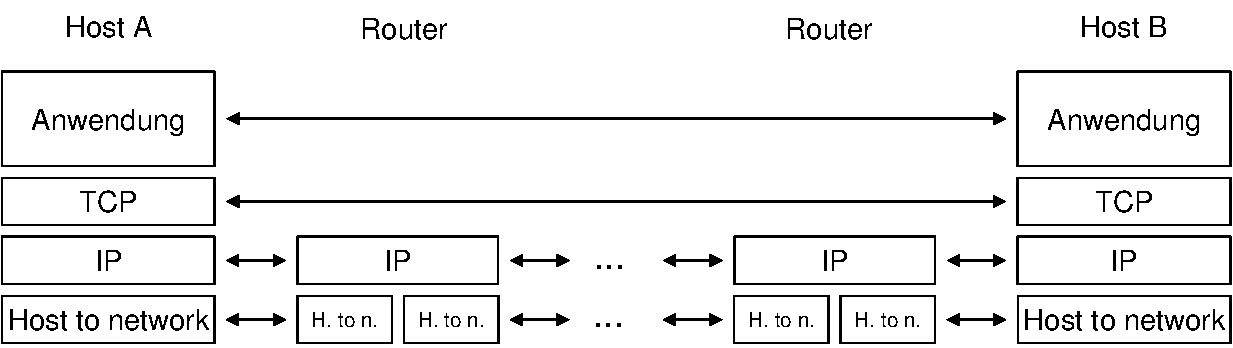
\includegraphics[width=\textwidth]{fig/communication}
%     \caption{The TCP/IP protocol stack during the communication process
%       between two hosts}%
%     \label{fig:1}
%   \end{center}
% \end{figure}



% \subsection{Figures of Other Authors}
% Lots of figures have been created, among them may even be figures that exactly match your work.
% If you find such a figure, you might want to use it in your paper/thesis.
% In this case you have to make a \textbf{figure reference} to the source of the figure; either in the figure itself or in the annex.

% If you wish to use a figure that is not available in an electronic format, the simplest of all solutions is to scan it.
% If the figure is part of an electronic document, you can make a screenshot.
% Mind that, using this type of figures, it is important to choose a sufficiently high resolution to ensure that the printer will not turn it into a load of \enquote{pixel mud}.
% At the same time, the resolution should be as low as possible in order to not unnecessarily blow up the size of the document.

% Therefore, it is worth considering drawing the picture yourself with a tool of your own preference and embed it as a \textbf{vector graphics}.
% In most of the cases you will end up having to apply changes to a foreign figure, because it eventually turns out to not 100\% match with the situation in your work.
% If after that the figure still strongly resembles the source, and if it is not a commonly well-known picture, as e.g.\ the TCP/IP protocol stack, the source must be marked as \enquote{[reference]}.
% We recommend choosing a vector format (\texttt{.wmf}, \texttt{.emf}, \texttt{.eps} und \texttt{.pdf}), since they do not occupy much space and scale arbitrarily without looking \enquote{pixelish}.


% \subsection{Colors}
% A colored figure is a nice thing --- provided you will use a color printer.
% In a black-and-white-print the colors will be reduced to their grades of brightness, as a result of which the contrast distribution will not remotely reach the intended quality.
% Therefore, when creating colored figures, make sure that even in a black-and-white print the necessary information will still be distinct.
% You can as well abstain from colors and use different shades of gray instead.
% In plots, different curves can be distinguished by using different line types.

% However, if you wish to use colored figures, do not refer to the colors in the text.
% Phrases like \enquote{Active nodes are marked red, passive nodes blue and inactive nodes green} in a black-and-white print have a rather comical effect and will lead to confusion rather than comprehension.

% \subsection{Plots}
% Plots should be created e.g.\ with Gnuplot~\cite{gnuplot_homepage}, R~\cite{r_homepage}, OpenOffice~\cite{oo_homepage}, or Excel.
% They can easily be embedded as vector formats, so it is not necessary to use screen shots.
% When using plots, it is important to \textbf{label all the axes} and indicate the \textbf{units}.

% Make sure to use an \textbf{appropriate scaling}.
% For example, instead of saying \enquote{10000000 bps} or \enquote{1.0e-07 bps} the more concise \enquote{10 Mbps} is preferable.

% An example of how not to do it is shown in \Cref{fig:plots} (a): a pixelish Gnuplot-screenshot without units at the axes and a badly chosen scale.
% Example (b) shows the same plot with a reasonable labeling as \texttt{.eps} import.

% \begin{figure}[ht]
%     \centering
%     \subfigure[Poor] {
%         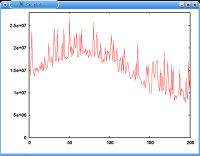
\includegraphics[width=9cm]{fig/plot_falsch_small}
%     }
%     \subfigure[Better] {
%         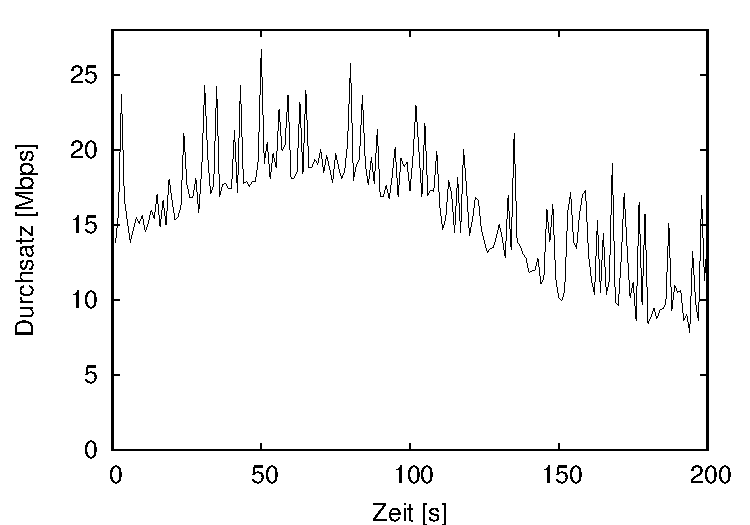
\includegraphics[width=9cm]{fig/plot_richtig}
%     }
%     \caption{Examples for a presentation of measurement results.}%
%     \label{fig:plots}
% \end{figure}


% \section{Tables}
% Most of the rules that apply to figures also apply for tables: Tables have to be numbered, captioned, and referenced in the text.
% The difference between tables and figures is that the caption is above the table but below a figure.
% In case you wish to present extensive measurement- or simulation results, a graphic representation may convey the information more concisely than a table.
% \Vref{tab:volume} provides a good example for table typesetting.



% \section{Code}
% \label{sec:code}
% It is often advisable to put complex algorithmic procedures in code.
% These shall be noted in \emph{Pseudocode} in natural language form.
% With regard to typesetting, the rules for figures (refer to \Cref{sec:figures}) apply to code, as well.
% A small example is given in \Cref{code:science}, below.

% \begin{algorithm}
%   \KwData{Your thesis task}
%   \KwResult{A thesis}

%   \While{not\_finished(thesis)}{
%     work\_on(thesis)\;
%   }
%   proofread(thesis)\;
%   turn\_in(thesis)\;

%   \caption{Pseudocode for compilation of a research thesis.}%
%   \label{code:science}
% \end{algorithm}

% This template includes the package \texttt{algorithm2e}~\cite{pkg:algorithm2e}.
% It is configured to the requirements outlined.

% \begin{lstlisting}[caption={Code example using lstlisting.},label=lstlisting]
%   // comments are never a bad idea
%   my_function()
%   {
%     float test1;
%     float test2;
%     test1 = some_function();
%     if (test1 > 0)
%           test2 = 0;
%     else
%           test2 = ((other_function(test1) * 10) / test1) * 100 ;
%     return test2;
%   }
% \end{lstlisting}

% The \texttt{lstlisting} environment may be an alternative if syntax is of importance.
% An example is depicted in \Cref{lstlisting}.


% \section{Quotations}
% \label{sec:quotations}
% We recommend to not extensively quote text sources.
% Computer scientists usually make it short; instead of quoting a source, they reference it in the appropriate place.
% However, it can be helpful to now and then quote a particular paragraph containing information which is crucial for your work.
% In this case, the quotation has to be put in \textbf{quotation marks} and stand out against the rest of the text (for example, by indented paragraphs or italicized font).
% Furthermore, the source has to be indicated by a reference (see quote from the MaPO in \Cref{sec:aufgaben-diplom}).

% By no means quotations may be used to describe the basics of your work.
% Although it is easy to find elaborate introductions to most subjects, it would by far miss the purpose of your work to simply adopt them.
% On the contrary, they can be rather incongruous since they most probably will not confine themselves to the essentials of this aspect of your work.

% If, in addition, the reference to the quotation is missing, it means that the author tries to pass off a foreign work as his own.
% This is called plagiarism and is incompatible with the methods of academic work which, as a purpose of our lectures, we want the students to acquire.

% \textbf{If we identify a case of plagiarism, we will get very angry --- sometimes angry to an extent that we will refuse the certificate, or grade the Master thesis as not passed.}


% \section{References}\label{sec:references}
% The following chapter addresses various aspects of referencing.

% \subsection{What do I reference?}
% When choosing a source, it is of great importance to check its reliability.
% Usually, the books, articles of scientific magazines or conference proceedings, standards, and other sources that we make available for you undergo a scientific review to ensure a certain reliability.

% Computer magazines, such as c't, iX etc., belong to a scientific twilight zone.
% They do get reviewed, however, the reviews are editorial, not scientific, hence they should be referenced for non-technical aspects only.
% For example, you should \emph{not} reference a TCP/IP-tutorial from the c't or, even worse, the Computer-Bild. More appropriate would be a reference to books or the relevant standards.
% However, in an introduction it is not at all out of place to quote from an article about the commercial predominance of a new radio communication standard and reference the sales figures for end devices mentioned in the article.

% You will need a good deal of skepticism when dealing with internet publications (including, among others, seminar/study papers from other authors) that were not obviously subject to review.
% You better avoid this kind of sources, since the internet makes it quite easy to publish the most amazing nonsense.


% \subsection{How do I reference?}
% Two different ways of referencing have been established.
% The first one are found mainly in English publications: The references are simply bracketed and serially numbered:

% \begin{example}
%   \subsubsection*{Example:}
%   An alternative mechanism for congestion control which recognizes congestion by the increase of round trip time was already introduced [1].
% \end{example}

% Alternatively, the signature of the reference consists of the initials of the authors' last names and the last 2 digits of the year of publication.
% This form of referencing is most customary in German publications:

% \begin{example}
%   \subsubsection*{Example:}
%   An alternative mechanism for congestion control which recognizes congestion by the increase of round trip time was already introduced [JWL04].
% \end{example}

% The following rules have proven useful for both notations:
% \begin{itemize}
%   \item To prevent a signature from getting too long, only the first
%     three authors will be mentioned. If there are more than three authors,
%     this is indicated by a \enquote{+} behind the list of authors
%     (e.g.\ [IML+01] for a paper published by Inamure, Montenegro, Ludwig,
%     Gurtov, and Khafizov in 2001).

%   \item In case there is only one author, the first three letters of his
%     last name will be indicated (e.g.\ [Hus01] for an article published by
%     Geoff Huston in 2001).

%   \item If an author or a group of authors produced more than one publication
%     in one year, the referenced publications of the same year will be distinguished by an attached lowercase letter (e.g.\ [Pos81a], [Pos81b] or [Pos81a,Pos81b]).

%   \item If there is no designated author or publisher (which can happen in case
%     of standards), arbitrarily choose an explicit letter combination (e.g.\ [IEEE99] for an IEEE standard).
% \end{itemize}

% When it comes to the point of where to set the reference specifically, please note that the reader would like to read a sentence of words he knows.
% The best choice is to phrase sentences that may be read without the reference itself.
% Please consider the following examples:

% \begin{example}
%   \subsubsection*{Example (poor):}
%   In [JWL04] we introduce an alternative mechanism for congestion control which recognizes congestion by the increase of round trip time.

%   \subsubsection*{Example (better):}
%   An alternative mechanism for congestion control which recognizes congestion by the increase of round trip time was already intrudeced [JWL04].
% \end{example}

% Further the specific place a reference is set does matter.
% The validity of the reference is limited to the next punctuation mark.
% If a reference is used before a full stop it is valid for this sentence.
% If it occurs behind a full stop, but right before the end of a paragraph.
% It is valid for the full paragraph.

% The references will be listed in a separate chapter at the end of the document.
% Each reference appears as a separate entry in the following format:

% \begin{example}
%   \begin{tabbing}
%     [Signature] \= author(s), title of publication, specification about magazine,
%     conference, \\ \> book in which the source was published, page number (if possible),\\
%     \> year of publication, ISBN.
%   \end{tabbing}
% \end{example}

% The information contained in the reference list has to be exhaustive enough to enable the reader to find the source (in fact, without using Google or Citeseer).


% \subsubsection*{Examples for RFCs/Standards:}
% \begin{example}
% \begin{tabbing}
%   {}[IEEE99] \= \kill \\
%   {}[Pos81a] \> J. Postel, \emph{Internet Protocol}, September 1981, IETF, RFC
%   791, Status: \\*
%   \> Standard.\\
%   {}[Pos81b] \> J. Postel, \emph{Transmission Control Protocol}, September
%   1981, IETF, RFC 793,\\*
%   \> Status: Standard.\\
%   {}[IEEE99] \> IEEE Computer Society LAN MAN Standards Committee,
%   \emph{Wireless LAN} \\*
%   \> \emph{Medium Access Control (MAC) and Physical Layer (PHY)
%   Specifications,} \\*
%   \> \emph{IEEE Std 802.11}, 1999 Edition, Institute of Electrical and
%   Electronics\\*
%   \> Engineers (IEEE), 1999.
% \end{tabbing}
% \end{example}

% \subsubsection*{Example for a Conference Paper}
% \begin{example}
% \begin{tabbing}
%   [JWL04] \= C. Jin, D. Wei, and S. Low, \emph{FAST TCP: Motivation,
%   Architecture,} \\*
%   \> \emph{Algorithms, Performance}, Proceedings of the 23rd Annual Joint
%   Conference \\*
%   \> of the IEEE Computer and Communications Societies, INFOCOM 2004,
%   \\*
%   \> March 2004.
% \end{tabbing}
% \end{example}


% \subsubsection*{Example for a Journal Article}
% \begin{example}
% \begin{tabbing}
%   [Hus01] \= G. Huston, \emph{Analyzing the Internet's BGP Routing Table},
%  The Internet\\*
%  \> Protocol Journal 4 (2001), no. 1, pp 2-15.
% \end{tabbing}
% \end{example}


% \subsubsection*{Example for a Website}
% \begin{example}
% \begin{tabbing}
%   [TCP03] \= Homepage of Tcptrace --- a tool for TCP trace Analysis, \\*
%   \> http://www.tcptrace.org, November 2003.
% \end{tabbing}
% \end{example}

% With a website reference it is obligatory to indicate the date of the reference, since websites are not usually static nor permanent.


% \subsubsection*{Example for a Book}
% \begin{example}
% \begin{tabbing}
%   [Ste94] \= W. R. Stevens, \emph{TCP/IP Illustrated: The Protocols}, vol. 1,
%   \\*
%   \> ISBN 0-201-63346-9, Addition Wesley 1994.
% \end{tabbing}
% \end{example}


% \subsection{BibTeX}
% When using the \emph{BibTeX} addition to \LaTeX{}, the signature is generated automatically, and you do not have to bother about their formats.
% In BibTeX, the references are managed in a separate .bib file, from which the necessary references will be extracted and embedded into the document by the \texttt{bibtex} command.
% References in BibTeX format are often available in the Web and save a lot of work.

% \section{Language}
% Generally, the language of a scientific research text should be neutral, matter-of-fact-ish, and not contain colloquial wording.
% After all, the reader of a scientific text wishes to receive precise information rather than to be entertained.

% \begin{example}
%   \subsubsection*{Example (poor):}
%   After a short while the sender wants to post the message again.

%   \subsubsection*{Example (better:)}
%   After 10 seconds the sender retries to transmit the message.
% \end{example}

% The \enquote{first person} should not be used in the type of elaborations discussed in this text.
% In German texts it is common to use the passive voice.
% In English texts you will often encounter the usage of \enquote{we}.

% \begin{example}
%   \subsubsection*{Example (poor):}
%   Therefore I decided to use solution XY.

%   \subsubsection*{Example (better):}
%   Therefore, we decided to implement solution XY. (\enquote{English style})

%   \subsubsection*{Example (possibly even better):}
%   Therefore, it was decided to implement solution XY. (\enquote{German style})
% \end{example}

% Generally, in a scientific text it is obligatory to substantiate all statements that are not obvious.
% This can be done by means of own research results (as, for example, in a Master thesis), or by referring to other sources providing either evidence or a logical and coherent motivation.

% During the writing process, the author should imagine himself in the place of the reader, making sure that he, being the reader, would still understand the text.
% It is a matter of course to write in full, grammatically correct sentences and avoid spelling mistakes.
% We highly recommend to use spell checkers (in \LaTeX{} e.g.\ GNU ispell~\cite{ispell_homepage}) and thoroughly proof-read the text at least once before handing it in.


% \section{Abbreviations}
% Please note that abbreviations and full text must not be mixed.
% When introducing an abbreviation for the first time, it should be written in full and the abbreviation attached in brackets.
% In the following text, only the abbreviation will be used.
% Common abbreviations can be applied without introducing them in full writing.

% \begin{example}
%   \subsubsection*{Example:}
%   The \gls{tcp} offers a reliable, connection-oriented transport service.
%   \gls{tcp} is \ldots
% \end{example}

% If a document contains a large amount of different abbreviations, it might be
% reasonable to summarize them in a list and attach it to the document.


% \section{Indices}
% If the volume of a document exceeds approximately 15 pages, it is advisable to generate a table of contents, for which every reasonable text system offers supportive tools.

% In voluminous documents, such as Master theses, separate indices of figures and tables are recommended.


% \section{Programming Code}
% To quote and discuss a voluminous programming code is one of the most effective means of boring your reader.
% In case you decide to introduce an algorithm, you will rather use a Pseudocode representation that confines itself to explaining the main functions of the algorithm.
% If a reader is interested in the implementation, they can refer to the actual programming code.
% For discussing data structures, UML class diagrams have proven quite useful.


% \section{Font Styles}
% \LaTeX{} supports multiple font styles.
% They might be used to accentuate a piece of text within a paragraph.
% This section is concerned with the application of the most common used styles.

% \textbf{Bold text} is often used to emphasize specific passages or terms.
% However, it disrupts the type face of a whole page.
% For this very reason it is recommended to refrain from its usage.

% \underline{Underlined text} is also only moderately beneficial.
% While screen reading, it appears to the reader like a hyper link, which is terribly misleading.
% In any case it disrupts the typeface, as well because it visually changes the line spacing.
% One should always prefer \textit{italics}.

% \texttt{Slated text} should be only used under very specific circumstances.
% It is suitable to accentuate words that differ in its meaning from the word in natural language.
% This is especially true when talking about commands of a program, programming language or a \texttt{shell}.

% \textit{Italic text} is best suited to accentuate text or term within continuous text.
% A lot of commands generate italic text in \LaTeX{}.
% \verb+\textit+, \verb+\emph+ or the mathematics environment (\verb+$$+) all generate italic text.
% Text should be emphasized especially when:

% \begin{enumerate}
%   \item A word is of a foreign language, like \emph{faux pas}.
%   \item An abbreviation is introduced, e.g.\ \emph{Transmission Control Protocol} (\emph{TCP}).
%   \item Something is of special meaning in this context \enquote{I will \emph{not}
%   make my supervisor angry.}
% \end{enumerate}

% \section{Multiple Authors}
% Project groups and Labs may be offered as a group work.
% This fact makes it important to make every paragraph attributable to a certain author.
% Only then is it possible to grade the participants fairly and corresponding to the particular accomplishments.
% If one is using this template for his work, the usage of the command \verb+\marginpar{Name}+ is heavily recommended.
% Appended to a paragraph it marks the authorship of that paragraph.
% \marginpar{Sykosch}

% \section{Definitions Theorems Remarks}
% In order to precisely pin down a definition, a statement or an example, you can use the environments mentioned below.

% \begin{definition}
%   A definition is used to pin down a family of objects.
%   Such a family is defined by a precise and compact specification of its features.
%   Then, an object is part of this family if and only if it possesses all the required features.
% \end{definition}


% \begin{remark}
%   Further explanations, remarks or examples are not part of a definition.
%   They can be part of surrounding environments like a \emph{remark} or an \emph{example}.
% \end{remark}


% \begin{theorem}
%   A theorem is a precisely formulated true statement.
% \end{theorem}


% \begin{proof}
%   This environment should be used to proof a claim.
% \end{proof}


% \begin{remark}
%   As before, further explanations, remarks or examples are not part of a theorem or a proof.
% \end{remark}
% \marginpar{Boes}



% \chapter{Conclusion}
% As a matter of fact, every piece of written academic work is subject to the individual criteria of their authors, characterizing their personal style of presenting facts.
% This style is not necessarily identical with the reader's personal concept of presentation; hence, it is most likely that some aspects of this guideline are based on our subjective idea of what characterizes a good composition.

% The majority of points mentioned in this guideline, however, reflect the practical values that have proven useful to us when presenting our own scientific texts.
% Therefore, it is worthwhile keeping this guideline in the back of your mind when composing your scientific work in order to avoid the grossest mistakes from the very beginning.
